\documentclass[12pt,a4paper]{article}

\usepackage[a4paper,margin=1in]{geometry}
\usepackage{graphicx}
\usepackage{listings}
\usepackage{xcolor}
\usepackage{titlesec}
\usepackage{longtable}
\usepackage{setspace}
\usepackage{times}

\usepackage{tikz}
\usetikzlibrary{shapes.geometric, arrows.meta, positioning}

\tikzstyle{block1} = [
rectangle,
rounded corners,
minimum width=6cm,
minimum height=1cm,
text centered,
draw=blue!70,
fill=blue!20,
thick
]

\tikzstyle{block2} = [
rectangle,
rounded corners,
minimum width=6cm,
minimum height=1cm,
text centered,
draw=green!60!black,
fill=green!20,
thick
]

\tikzstyle{block3} = [
rectangle,
rounded corners,
minimum width=6cm,
minimum height=1cm,
text centered,
draw=orange!80!black,
fill=orange!25,
thick
]

\tikzstyle{block4} = [
rectangle,
rounded corners,
minimum width=6cm,
minimum height=1cm,
text centered,
draw=red!70!black,
fill=red!20,
thick
]

\tikzstyle{arrow} = [
thick,
-{Stealth[length=3mm]},
draw=black!80
]

\lstset{
	basicstyle=\ttfamily\small,
	keywordstyle=\color{blue},
	commentstyle=\color{codegreen},
	stringstyle=\color{red},
	breaklines=true,
	frame=single
}

\titleformat{\section}
{\large\bfseries}
{\thesection.}{0.5em}{}

\begin{document}
	
	\begin{titlepage}
		
		\centering
		
		\vspace*{1cm}
		
		{\Huge \textbf{MINI-PROJECT REPORT} \par}
		
		\vspace{2cm}
		
		{\LARGE \textbf{Packet-Level Traffic Analysis for Anomaly Detection using Wireshark} \par}
		
		\vspace{3cm}
		
		{\Large Submitted by \par}
		
		\vspace{0.7cm}
		
		{\Large \textbf{Anbuselvi. S } \par}
		
		\vspace{0.3cm}
		
		{\large  25237197207 \par}
		
		\vspace{2cm}
		
		{\Large \textbf{Course Name:} Artificial Intelligence for Cybersecurity \par}
		
		\vspace{0.5cm}
		
		{\Large \textbf{Course Code:} CB3201 \par}
		
		\vfill
		
		\vspace{0.5cm}
		
		{\large DEPARTMENT OF COMPUTER SCIENCE AND ENGINEERING \par}
		{\large COLELGE OF ENGINEERING GUINDY \par}
		{\large ANNA UNIVERSITY  \par}
		
		\vspace{1cm}
		
		{\large May 2026 \par}
		
	\end{titlepage}
	
	
	\vspace{0.5cm}

	\section{Objective}
	
	\begin{itemize}
		\item To capture and analyze network packets using Wireshark and tshark.
		\item To detect abnormal network traffic patterns using Machine Learning techniques.
		\item To build a real-time anomaly detection dashboard using Streamlit.
		\item To identify suspicious traffic such as packet bursts, oversized packets, and abnormal traffic behavior.
	\end{itemize}
	
	\section{Tool(s) Used}
	
	\begin{longtable}{|p{5cm}|p{8cm}|}
		\hline
		\textbf{Tool} & \textbf{Purpose} \\ \hline
		Wireshark & Packet capture and protocol analysis \\ \hline
		tshark & CLI-based packet feature extraction \\ \hline
		Python & Data processing and ML \\ \hline
		Pandas and NumPy & Feature engineering \\ \hline
		Scikit-learn & Isolation Forest anomaly detection \\ \hline
		Streamlit & Real-time dashboard \\ \hline
		Plotly & Interactive visualization \\ \hline
	\end{longtable}
	
	\section{Hardware Requirements}
	
	The following hardware configuration is recommended for efficient packet capturing, traffic processing, and anomaly detection.
	
	\begin{itemize}
		\item \textbf{Processor} : Intel Core i5 / AMD Ryzen 5 or above
		\item \textbf{RAM} : Minimum 8 GB
		\item \textbf{Storage} : At least 10 GB free disk space
		\item \textbf{Network Adapter} : Ethernet or WiFi Interface Card
		\item \textbf{Display} : Minimum 1366 $\times$ 768 resolution
		\item \textbf{Operating System} : Ubuntu Linux / Windows / macOS
	\end{itemize}
	
	The hardware configuration should support live packet capturing, real-time dashboard visualization, and machine learning-based anomaly detection without significant performance degradation.
	\newpage
	\section{Software Setup}
	
	This section describes the installation and configuration steps required to set up the environment for packet-level traffic analysis and anomaly detection.
	
	\subsection*{Required Software}
	
	\begin{itemize}
		\item Python 3.10 or above
		\item Wireshark
		\item tshark
		\item Streamlit
		\item Nmap
	\end{itemize}
	
	\vspace{0.02cm}
	
	\subsection*{Step 1 -- Install Python}
	
	Install Python 3.10 or above from the official Python website.
	
	\begin{center}
		\texttt{https://www.python.org/downloads/}
	\end{center}
	
	Verify the installation using:
	
	\begin{lstlisting}[language=bash]
		python3 --version
	\end{lstlisting}
	
	\vspace{0.5cm}
	
	\subsection*{Step 2 -- Install Wireshark and tshark}
	
	Install Wireshark and tshark using the following commands:
	
	\begin{lstlisting}[language=bash]
		sudo apt update
		sudo apt install wireshark tshark
	\end{lstlisting}
	
	Verify tshark installation:
	
	\begin{lstlisting}[language=bash]
		tshark -v
	\end{lstlisting}
	
	\vspace{0.5cm}
	
	\subsection*{Step 3 -- Install Nmap}
	
	Install Nmap for generating scanning traffic used in anomaly detection.
	
	\begin{lstlisting}[language=bash]
		sudo apt install nmap
	\end{lstlisting}
	
	Verify installation:
	
	\begin{lstlisting}[language=bash]
		nmap --version
	\end{lstlisting}
	
	\vspace{0.5cm}
	
	\subsection*{Step 4 -- Create Python Virtual Environment}
	
	Create and activate a virtual environment for the project.
	
	\begin{lstlisting}[language=bash]
		python3 -m venv venv
		source venv/bin/activate
	\end{lstlisting}
	
	\vspace{0.5cm}
	
	\subsection*{Step 5 -- Install Required Python Libraries}
	
	Install all required Python libraries using pip.
	
	\begin{lstlisting}[language=bash]
		pip install pandas numpy scikit-learn \
		streamlit plotly matplotlib
	\end{lstlisting}
	
	\vspace{0.5cm}
	
	\subsection*{Step 6 -- Project Files Setup}
	
	Place the following files inside the project directory:
	
	\begin{itemize}
		\item \texttt{app.py}
		\item \texttt{attack.pcapng}
		\item \texttt{features.csv}
		\item \texttt{requirements.txt}
	\end{itemize}
	
	\vspace{0.5cm}
	
	\subsection*{Step 7 -- Run the Streamlit Dashboard}
	
	Execute the Streamlit application using:
	
	\begin{lstlisting}[language=bash]
		streamlit run app.py
	\end{lstlisting}
	
	After execution, the dashboard will be available in the browser at:
	
	\begin{center}
		\texttt{http://localhost:8502}
	\end{center}
	
	\vspace{0.5cm}
	
	\subsection*{Step 8 -- Verify Successful Setup}
	
	The dashboard should display:
	
	\begin{itemize}
		\item Traffic activity timeline
		\item Suspicious hosts
		\item Packet statistics
		\item ML-based anomaly detection results
		\item Packet size distribution graphs
	\end{itemize}
	\section{Architecture / Flow Diagram}
	
	\subsection*{System Workflow}
	
	\begin{figure}[h]
		\centering
		
		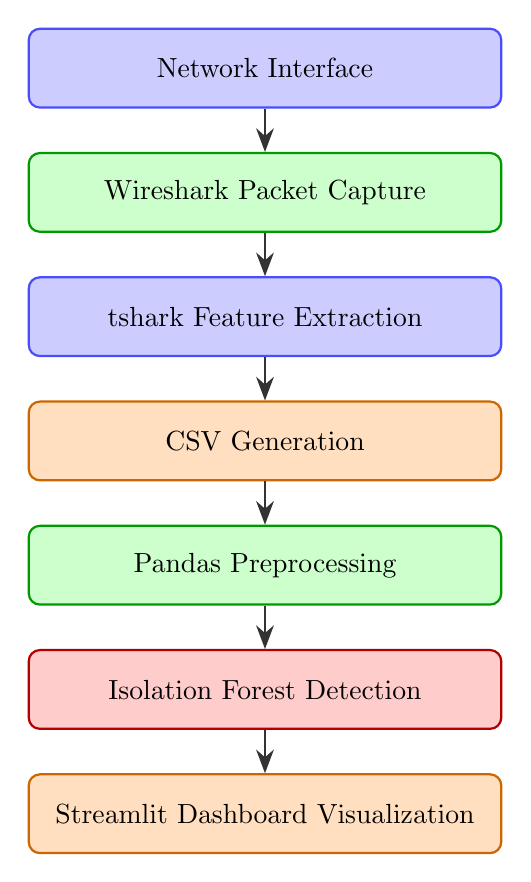
\begin{tikzpicture}[node distance=0.55cm]
			
			\node (n1) [block1] {Network Interface};
			
			\node (n2) [block2, below=of n1] {Wireshark Packet Capture};
			
			\node (n3) [block1, below=of n2] {tshark Feature Extraction};
			
			\node (n4) [block3, below=of n3] {CSV Generation};
			
			\node (n5) [block2, below=of n4] {Pandas Preprocessing};
			
			\node (n6) [block4, below=of n5] {Isolation Forest Detection};
			
			\node (n7) [block3, below=of n6] {Streamlit Dashboard Visualization};
			
			\draw [arrow] (n1) -- (n2);
			\draw [arrow] (n2) -- (n3);
			\draw [arrow] (n3) -- (n4);
			\draw [arrow] (n4) -- (n5);
			\draw [arrow] (n5) -- (n6);
			\draw [arrow] (n6) -- (n7);
			
		\end{tikzpicture}
		
		\caption{Packet-Level Traffic Analysis and Anomaly Detection Workflow}
		
	\end{figure}
	
	\section{Algorithm / Working Procedure}
	
	\subsection*{Step 1 -- Packet Capture}
	
	Wireshark captures live packets from the network interface.
	
	\subsection*{Step 2 -- Feature Extraction}
	
	tshark extracts packet fields into CSV format.
	
	\begin{lstlisting}[language=bash]
		tshark -r capture.pcapng -T fields \
		-e frame.number \
		-e frame.time_relative \
		-e ip.src \
		-e ip.dst \
		-e tcp.srcport \
		-e tcp.dstport \
		-e frame.len \
		-E header=y \
		-E separator=, \
		> features.csv
	\end{lstlisting}
	
	\subsection*{Step 3 -- Data Preprocessing}
	
	\begin{itemize}
		\item Remove null values
		\item Convert timestamps
		\item Generate traffic features
	\end{itemize}
	
	\subsection*{Step 4 -- ML-Based Detection}
	
	Isolation Forest detects abnormal traffic behavior.
	
	\begin{lstlisting}[language=Python]
		model = IsolationForest(
		n_estimators=200,
		contamination=0.01,
		random_state=42)
	\end{lstlisting}
	
	\subsection*{Step 5 -- Traffic Spike Detection}
	
	Packets are resampled into 1-second bins to detect abnormal traffic bursts.
	
	\begin{lstlisting}[language=Python]
		pps = df.resample("1s").size()
	\end{lstlisting}
	
	\subsection*{Step 6 -- Visualization}
	
	Results are displayed using Streamlit dashboards:
	
	\begin{itemize}
		\item Traffic spikes
		\item Top talkers
		\item Packet size histogram
		\item ML anomalies
		\item PPS graphs
	\end{itemize}
	
	\section{Use Cases}
	
	\begin{itemize}
		
		\item \textbf{Enterprise SOC} -- Continuous monitoring of enterprise network traffic and detection of suspicious and anomalous activities.
		
		\item \textbf{Academic Research} -- Network traffic dataset generation and machine learning-based traffic analysis.
		
		\item \textbf{IoT Security} -- Detection of rogue IoT devices and monitoring abnormal IoT communication.
		
		\item \textbf{Digital Forensics} -- Post-incident packet analysis and reconstruction of attack timelines.
		
		\item \textbf{Education and Labs} -- Cybersecurity practical training and packet-level traffic analysis learning.
		
	\end{itemize}
	
	\section{Step-by-Step Execution with Result Screenshots}
	
	\subsection*{Step 1 -- Capture Packets}
	
	Open Wireshark and select the active network interface such as \texttt{eth0} or \texttt{wlan0} to begin live packet capturing.
	
	\begin{center}
		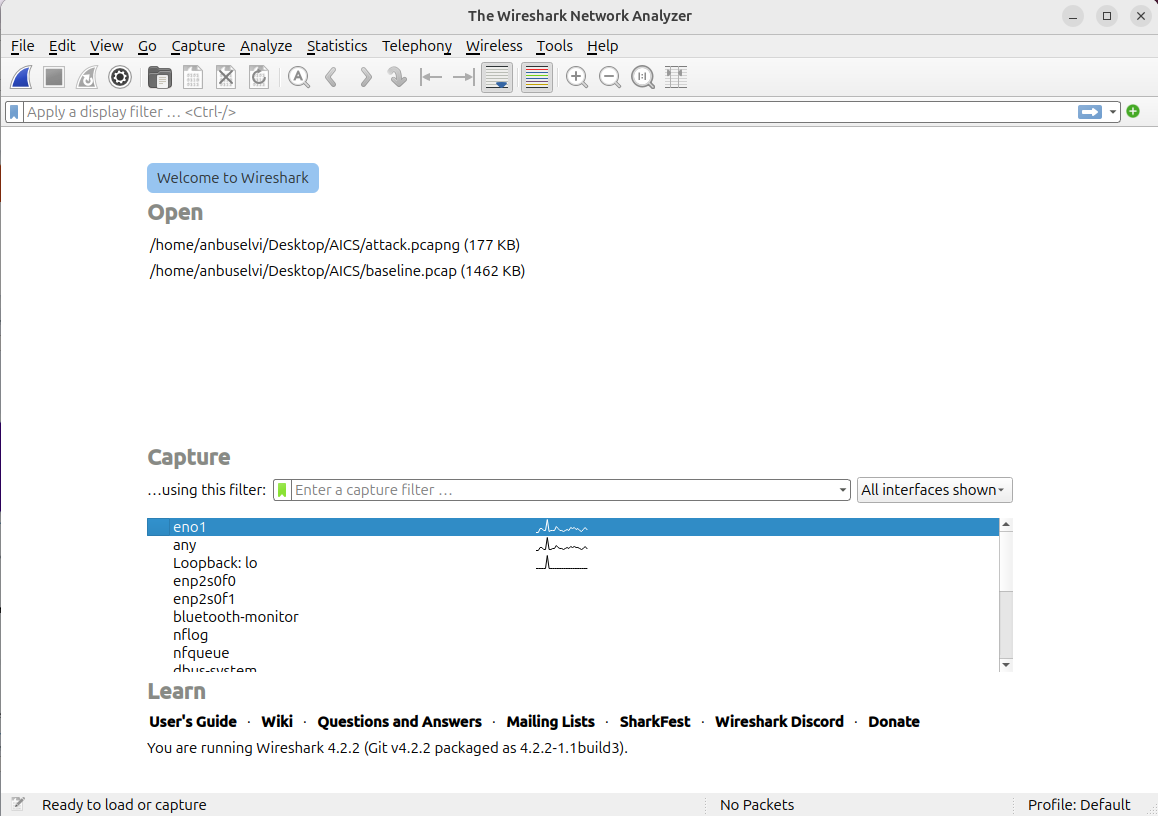
\includegraphics[width=0.7\textwidth]{1.png}
	\end{center}
	
	\begin{center}
		\textbf{Figure 1: Wireshark Interface Selection Window}
	\end{center}
	
	The Wireshark home screen displays all available network interfaces for capturing packets.
	
	\begin{center}
		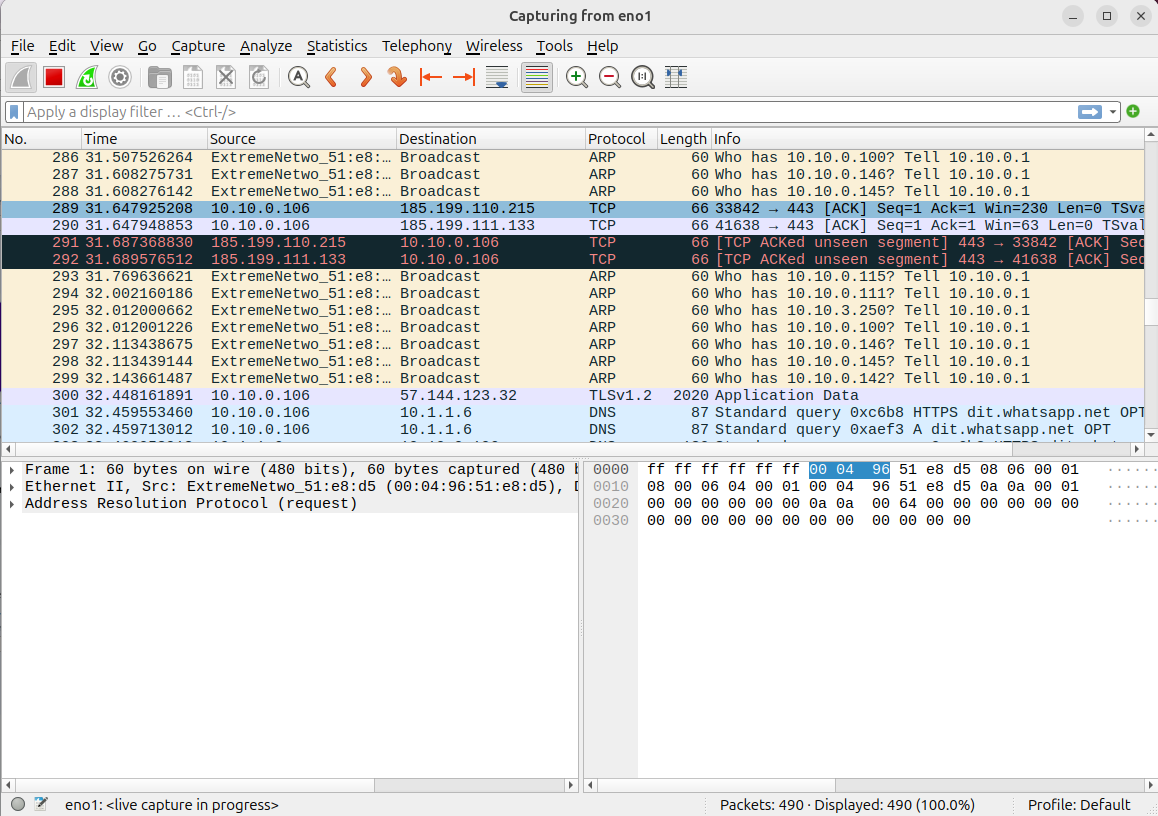
\includegraphics[width=0.75\textwidth]{2.png}
	\end{center}
	
	\begin{center}
		\textbf{Figure 2: Live Packet Capture in Wireshark}
	\end{center}
		
	Live network packets captured from the selected interface are displayed with protocol, source, destination, and packet details.
	
	\clearpage
	
	\subsection*{Step 2 -- Generate Traffic}
	
	Nmap commands are executed to generate scanning and reconnaissance traffic for anomaly analysis.
	
	\begin{center}
		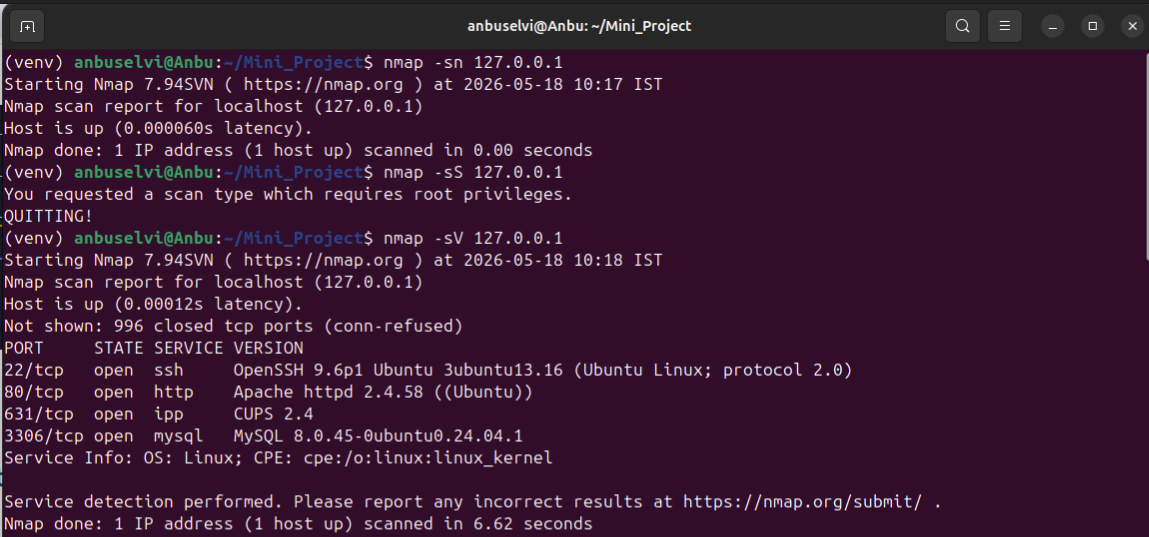
\includegraphics[width=0.85\textwidth]{3.1.png}
	\end{center}
	
	\begin{center}
		\textbf{Figure 3: Nmap Host Discovery Scan}
	\end{center}
	
	The host discovery scan checks whether the target system is active and reachable.
	
	\vspace{0.5cm}
	
	\begin{center}
		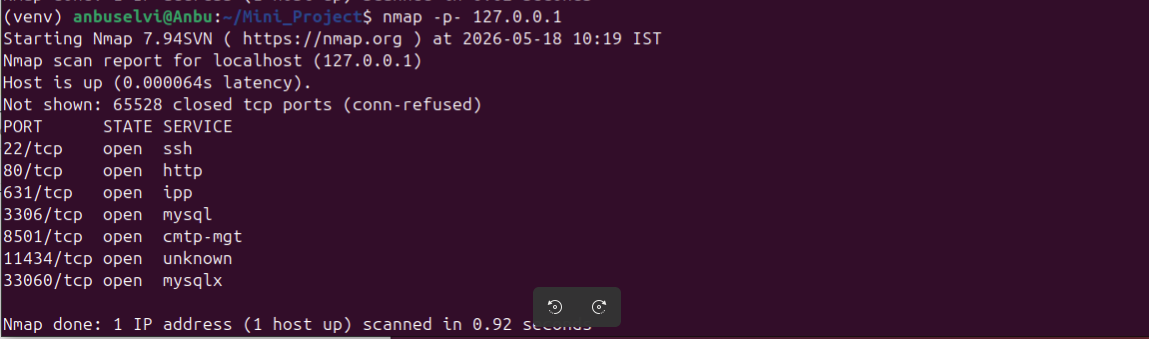
\includegraphics[width=0.85\textwidth]{3.2.png}
	\end{center}
	
	\begin{center}
		\textbf{Figure 4: Nmap Full Port Scan Results}
	\end{center}
	
	The full port scan identifies open ports and active services running on the target system.
	
	\clearpage
	
	\subsection*{Step 3 -- Stop and Save Captured Packets}
	
	After traffic generation, the captured packets are saved in \texttt{.pcapng} format for offline analysis.
	
	\begin{center}
		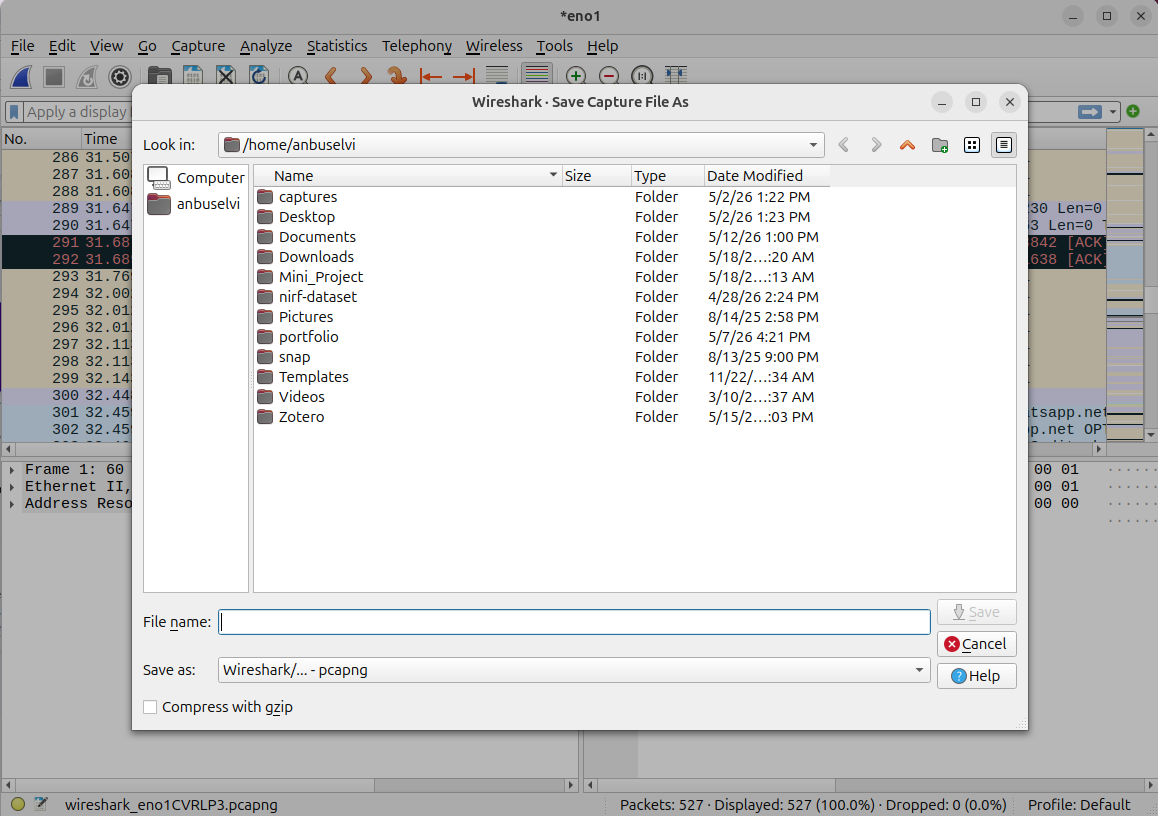
\includegraphics[width=0.85\textwidth]{4.png}
	\end{center}
	
	\begin{center}
		\textbf{Figure 5: Saving Captured Packets as PCAPNG File}
	\end{center}
	
	Wireshark provides options to save captured traffic files for future packet analysis and feature extraction.
	
	\vspace{0.6cm}
	
	\subsection*{Step 4 -- Export Features}
	
	tshark extracts packet-level features from the capture file and stores them in CSV format.
	
	\begin{center}
		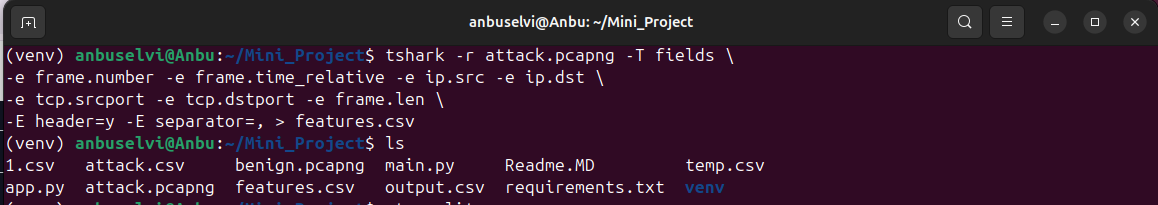
\includegraphics[width=0.85\textwidth]{5.png}
	\end{center}
	
	\begin{center}
		\textbf{Figure 6: tshark Feature Extraction Command Execution}
	\end{center}
	
	Packet attributes such as source IP, destination IP, ports, and packet length are exported into a CSV dataset.
	
	\clearpage
	
	\subsection*{Step 5 -- Run Detection Dashboard}
	
	The Streamlit application is executed to launch the anomaly detection dashboard.
	
	\begin{center}
		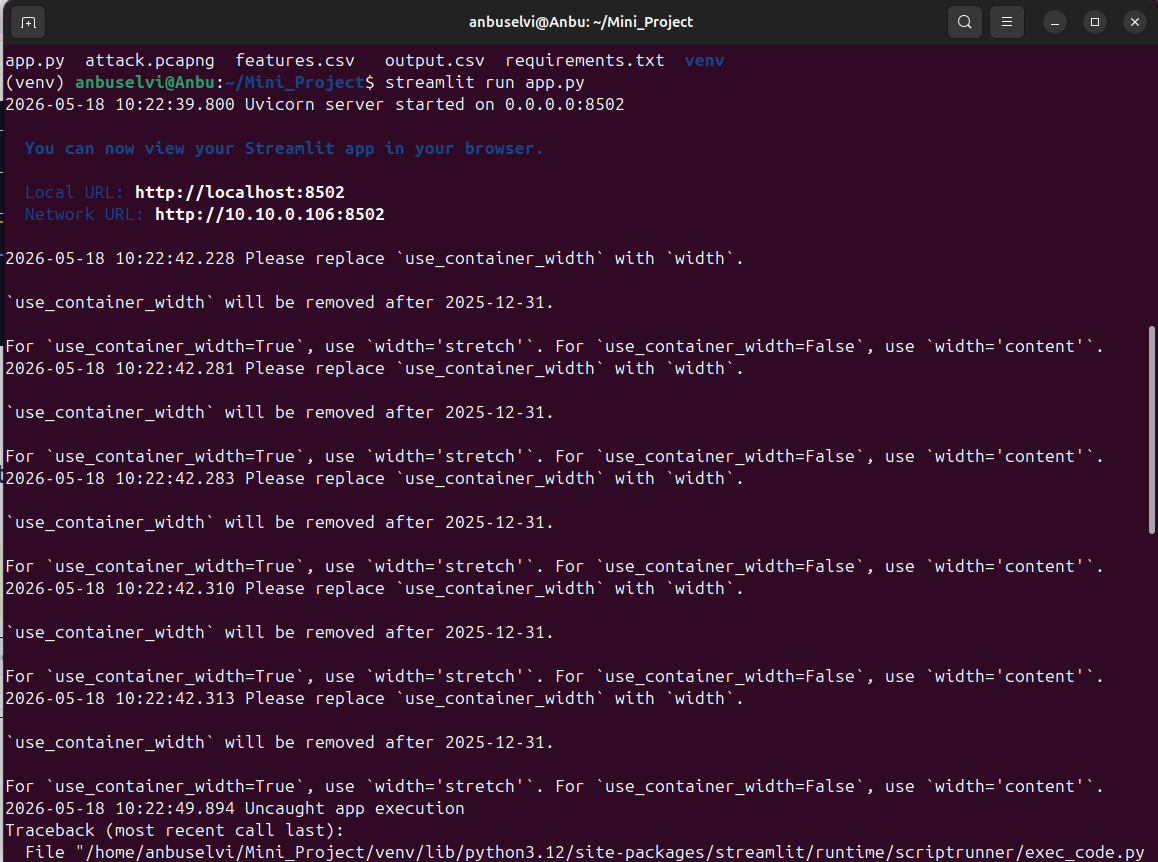
\includegraphics[width=0.75\textwidth]{6.png}
	\end{center}
	
	\begin{center}
		\textbf{Figure 7: Running Streamlit Detection Dashboard}
	\end{center}
	
	The Streamlit server initializes the real-time dashboard for network traffic visualization and anomaly monitoring.
	
	\vspace{0.2cm}
	
	\subsection*{Step 6 -- Observe Dashboard Results}
	
	The dashboard visualizes anomalies, suspicious hosts, packet statistics, and traffic behavior.
	
	\begin{center}
		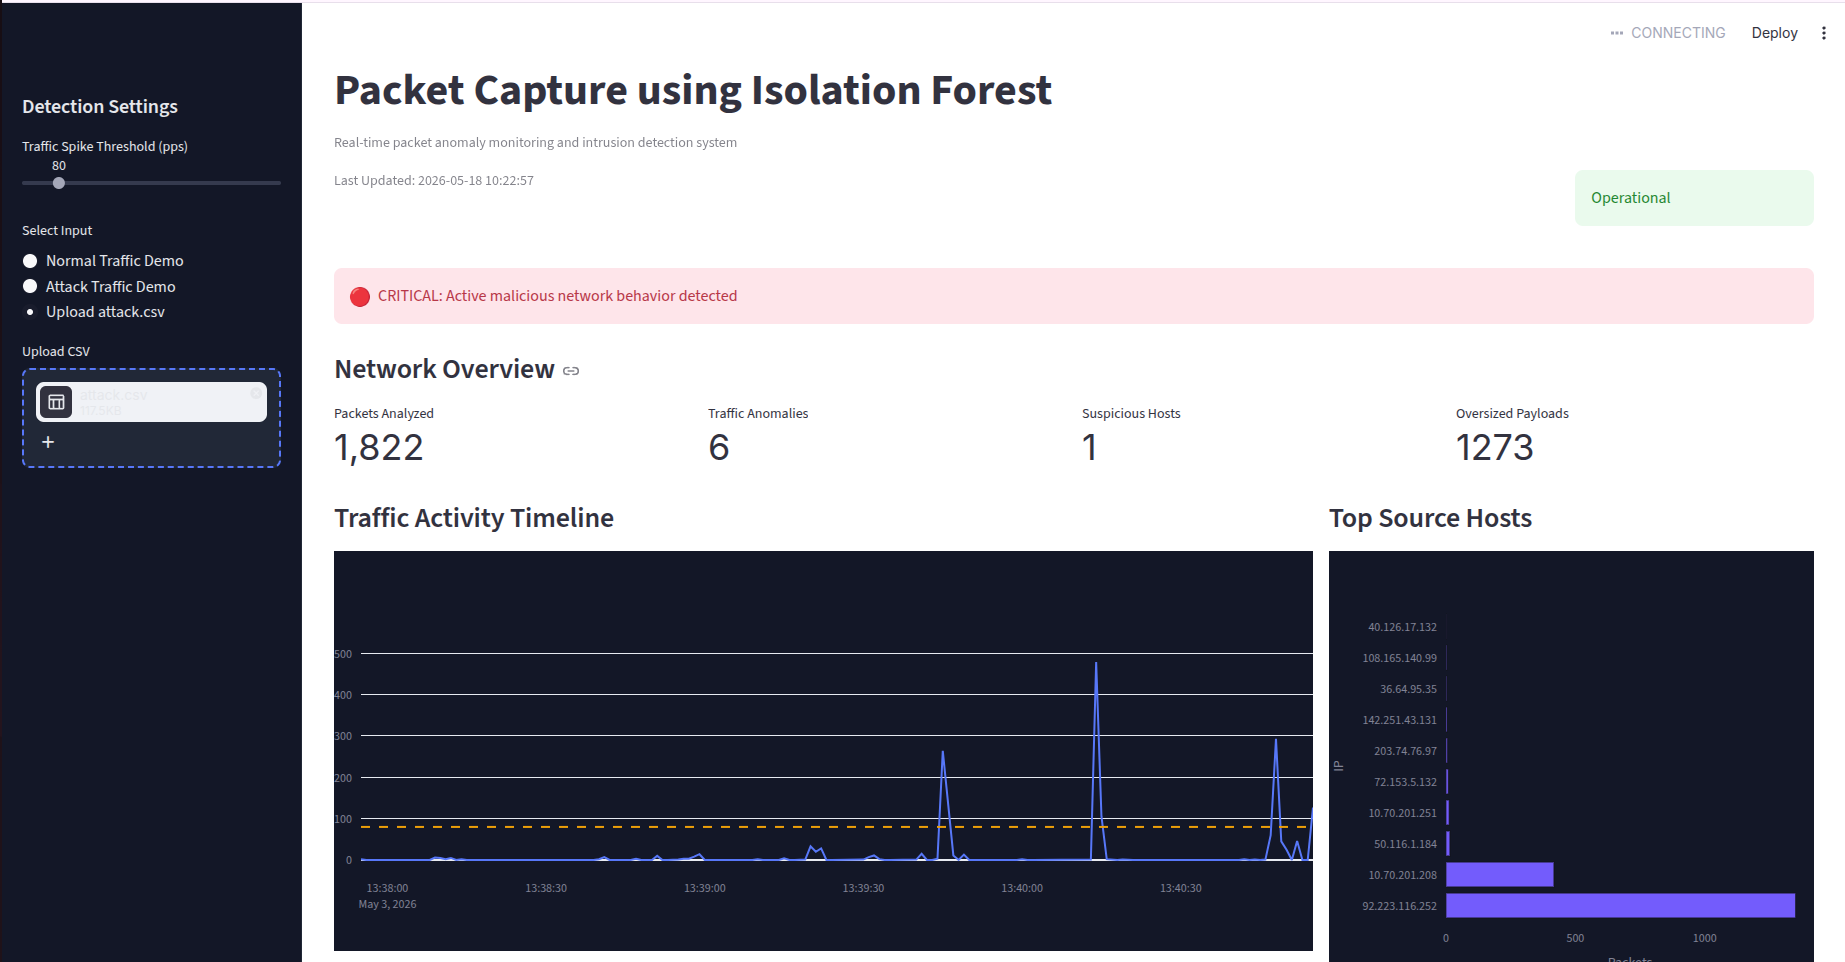
\includegraphics[width=0.8\textwidth]{7.png}
	\end{center}
	
	\begin{center}
		\textbf{Figure 8: ML-Based Threat Analysis Dashboard}
	\end{center}
	
	The dashboard identifies anomalous hosts and oversized payload events using Isolation Forest.
	
	\vspace{0.5cm}
	
	\begin{center}
		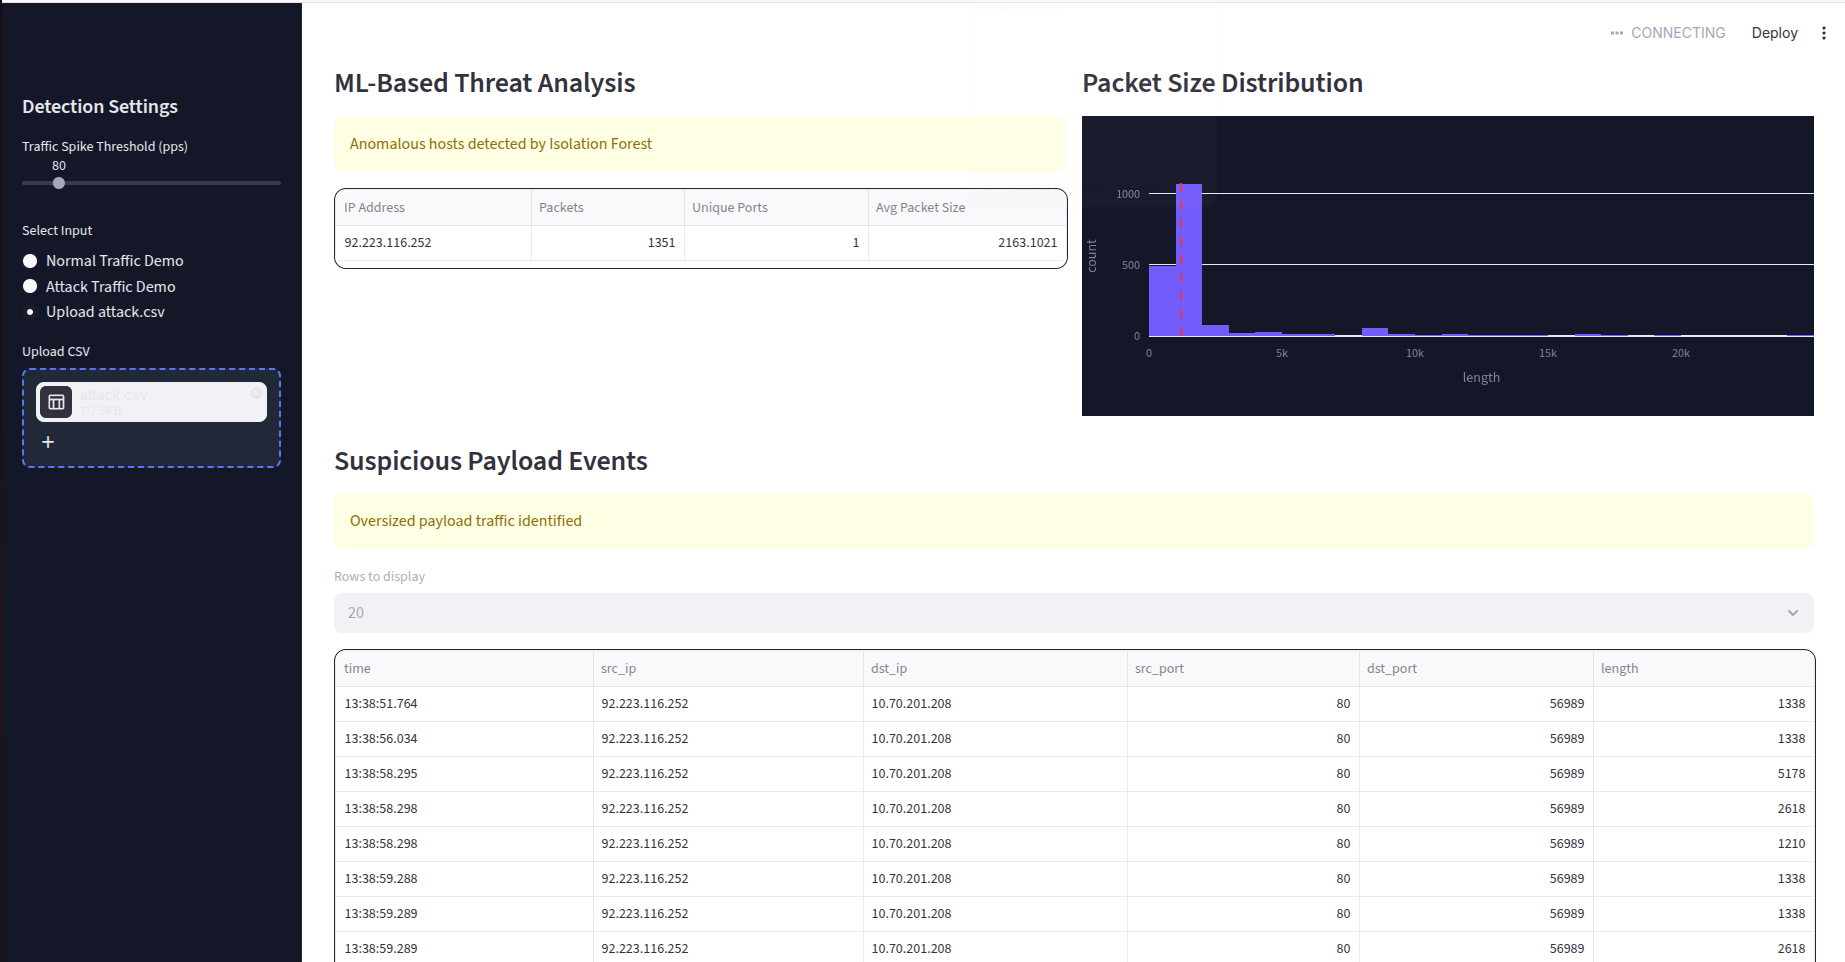
\includegraphics[width=0.85\textwidth]{8.png}
	\end{center}
	
	\begin{center}
		\textbf{Figure 9: Real-Time Network Traffic Monitoring Dashboard}
	\end{center}
	
	Traffic activity timelines and top source hosts are displayed for continuous monitoring.
	
	\vspace{0.85cm}
	
	\begin{center}
		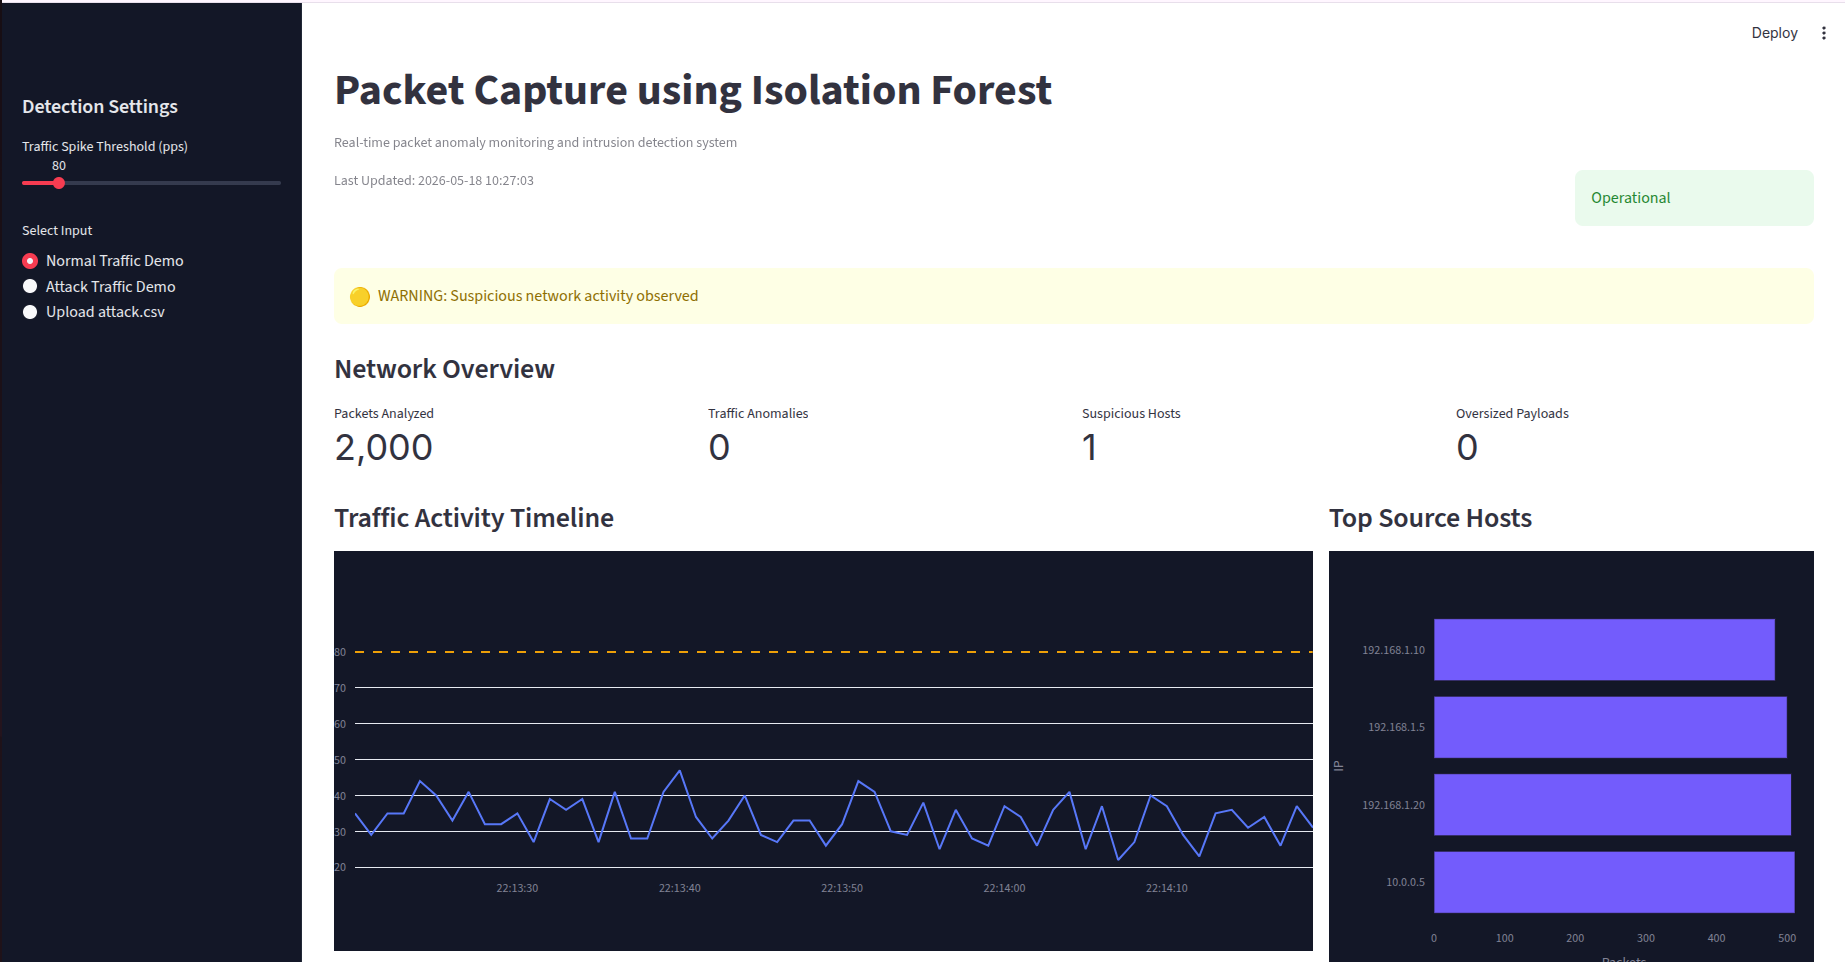
\includegraphics[width=0.85\textwidth]{9.png}
	\end{center}
	
	\begin{center}
		\textbf{Figure 10: Normal Traffic Detection Results}
	\end{center}
	
	The dashboard displays normal traffic behavior with minimal anomalies detected.
	
	\vspace{0.85cm}
	
	\begin{center}
		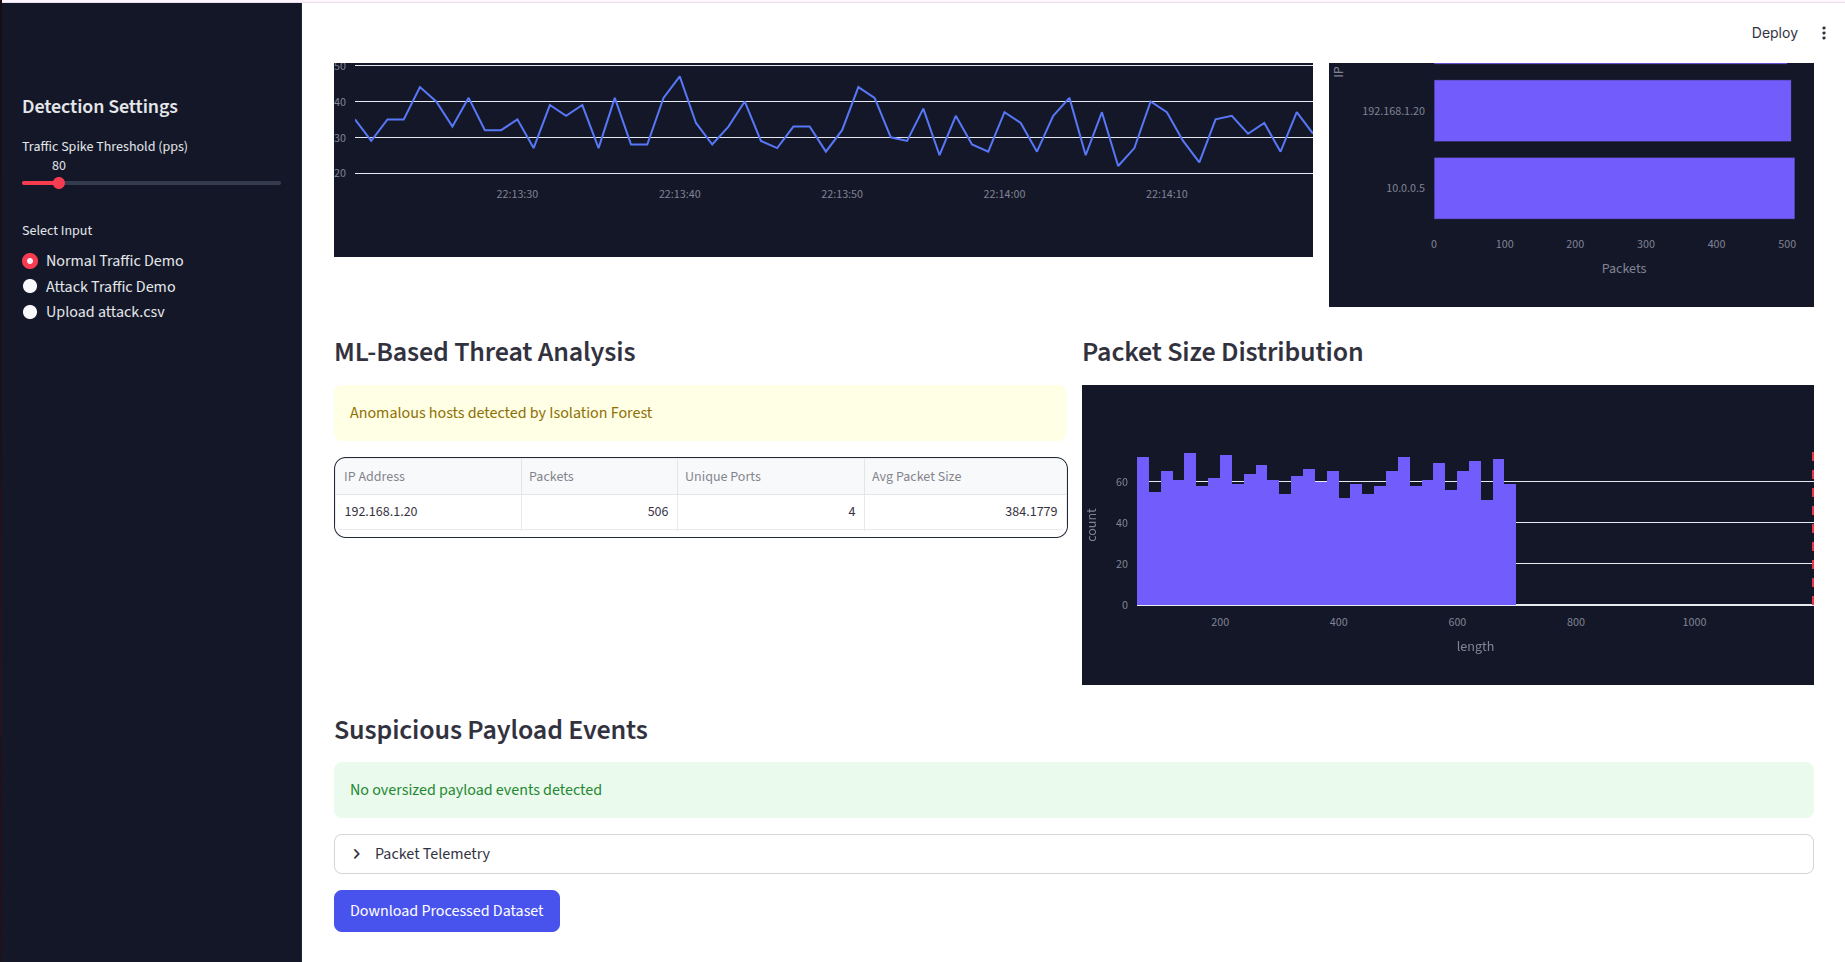
\includegraphics[width=0.7\textwidth]{10.png}
	\end{center}
	
	\begin{center}
		\textbf{Figure 11: Packet Size Distribution and Threat Analysis}
	\end{center}
	
	Packet size distribution graphs help visualize suspicious packet payload activity and abnormal traffic behavior.
	
	\vspace{0.25cm}
	
	\subsection*{Step 7 -- Downloaded CSV File}
	
	The processed packet-level traffic dataset is exported and stored in CSV format.
	
	\begin{center}
		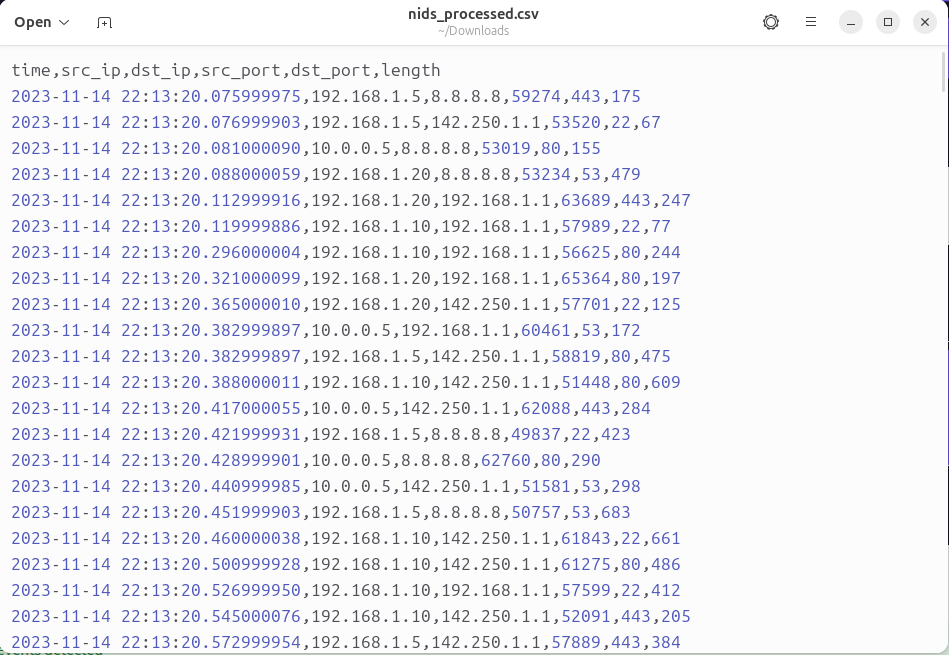
\includegraphics[width=0.65\textwidth]{11.png}
	\end{center}
	
	\begin{center}
		\textbf{Figure 12: Extracted Packet Features in CSV Format}
	\end{center}
	
	The CSV file contains extracted packet features used for anomaly detection and traffic analysis.
	
	\vspace{0.5cm}
	
	\section{Conclusion}
	
	This project successfully demonstrated packet-level anomaly detection using Wireshark, tshark, Machine Learning, and Streamlit. Packet features were extracted and analyzed to identify abnormal traffic behavior such as traffic spikes and oversized packets. Isolation Forest enabled ML-based anomaly detection, while Streamlit provided real-time visualization and monitoring. The workflow provides a scalable and low-cost solution for network traffic analysis and cybersecurity monitoring.
	
\end{document}